\documentclass[tikz, border=2pt]{standalone}
\usepackage{amsmath}

\begin{document}
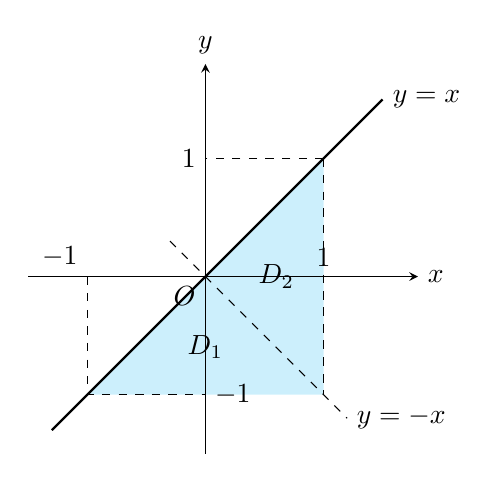
\begin{tikzpicture}[scale=1.5, >=stealth]
    % 填充积分区域 D (三角形：顶点为 (-1,-1), (1,-1), (1,1))
    \fill[cyan!20] (-1,-1) -- (1,-1) -- (1,1) -- cycle;

    % 画坐标轴
    \draw[->] (-1.5, 0) -- (1.8, 0) node[right] {$x$};
    \draw[->] (0, -1.5) -- (0, 1.8) node[above] {$y$};

    % 画直线 y = x
    \draw[thick] (-1.3, -1.3) -- (1.5, 1.5) node[right] {$y=x$};
    \draw[dashed] (-0.3, 0.3) -- (1.2, -1.2) node[right] {$y=-x$};

    % 画边界辅助线
    \draw[dashed] (-1, 0) node[above left] {$-1$} -- (-1, -1) -- (0, -1) node[right] {$-1$};
    \draw[dashed] (1, 1) -- (0, 1) node[left] {$1$};
    \draw[dashed] (1, 1) -- (1, -1) -- (1, 0) node[above] {$1$};

    % 标注区域 D 和原点
    \node at (0, -0.6) {$D_1$};
    \node at (0.6, 0) {$D_2$};
    \node[below left] at (0,0) {$O$};
\end{tikzpicture}
\end{document}